% Template for ICIP-2019 paper; to be used with:
%          spconf.sty  - ICASSP/ICIP LaTeX style file, and
%          IEEEbib.bst - IEEE bibliography style file.
% --------------------------------------------------------------------------
\documentclass{article}
\usepackage{spconf,amsmath,graphicx,titlesec}

    
% Example definitions.
% --------------------
\def\x{{\mathbf x}}
\def\L{{\cal L}}


% Title.
% ------
\title{ISSM report, Police Alert System}
%
% Single address.
% ---------------
\name{NG SIEW PHENG, TEA LEE SENG, YANG XIAOYAN	}
\address{Institute of Systems Science, National University of Singapore, Singapore 119615}

\begin{document}
%\ninept
%
\maketitle
%
\begin{abstract}
% Briefly describe your problem statement and the proposed approach.

Singapore is a safe country. However, any gun shots become more dangerous in neighbourhood area, due to less awareness in public. It is critical to maintain safety here and automate alerting mechanism to Police will be time and life saving. 
We propose machine learning mechanism to understand background sound in Urban setup to identify gun shots. We apply techniques like 1D conv neural network, auto-encoder, LSTM, neural network on MFCC to understand which is good for recognizing gun shots in URBANSOUND8K DATASET.
 

\end{abstract}
%
\begin{keywords}
URBANSOUND8K DATASET, long short-term memory, auto encoder, mfcc, conv1D, MaxPooling1D, deep neural network, deep learning
\end{keywords}
%
\section{Introduction}
\label{sec:intro}
% Describe the problem you are working on and why it is important. 


Dangerous weapons can be a source of dangerous in a safe country.  Gun shots become more dangerous in neighbourhood area, due to less awareness in public. It is critical to maintain safety here and automate alerting mechanism to Police will be time and life saving. It is easpecially the case that police station may be far away from the incident area and they do not get alerted unless civilians reported it to them. Even with reports, the actual sound about the incident is lost and therefore losing original data.


% \begin{itemize}
%  \item The main report is provided in *.tex file
%  \item The reference is provided in *.bib file
%  \item The figures are provided as separate jpg/png files
% \end{itemize}


\section{Related work}

% Discuss published works or online references that relate to your project, such as \cite{adams1995hitchhiker}
% \cite{MikeSmalesSoundClassificationusingDeepLearning}

We download URBANSOUND8K DATASET from \cite{URBANSOUND8K-DATASET} for analysis and classification models training. URBANSOUND8K DATASET was processed for \cite{Salamon:UrbanSound:ACMMM:14} research.


We also refer to Ricky Kim's articles about UrbanSound Classification Part 1 \cite{RickyKimUrbanSoundClassificationPart1soundwavedigitalaudiosignal} and Part 2 \cite{RickyKimUrbanSoundClassificationPart2samplerateconversionLibrosa} for initial understanding of datasets. 

Mike's work \cite{MikeSmalesSoundClassificationusingDeepLearning} on 2d convolution deep neural network on MFCC also share us another direction on utilizing frequency domain representation for analysis. 


\section{Proposed approach}
\label{sec:proposed approach}
Based on the nature that all sounds wave files are 1 dimensional signals, sampling at different frequencies, we retrieved wave data via librosa library at default 22khz sampling rate.

We concatenates signals itself to 4 seconds long as signal feature.

We feed the signals to conv1d, auto-encoder, and LSTM networks for classification.

we also convert signals to mfcc representation, apply mean on each mfcc stream and 3 layers dense neural network for classification.

Please refers experimental results section for details.


\label{sec:experimental results}
\section{Data preprocessing and analysis}
URBANSOUND8K DATASET\cite{URBANSOUND8K-DATASET} contains 8732 labeled sounds of 10 classes:
air\_conditioner, car\_horn, children\_playing, dog\_bark, drilling, enginge\_idling, gun\_shot, jackhammer, siren, and street\_music.
The sounds are of various sampling rate as well as sampling rate. We utilize librose to convert sampling rate to 22kHz and mono channel. 

\begin{figure}[h]
	\centerline{\begin{tabular}{cc|c}
			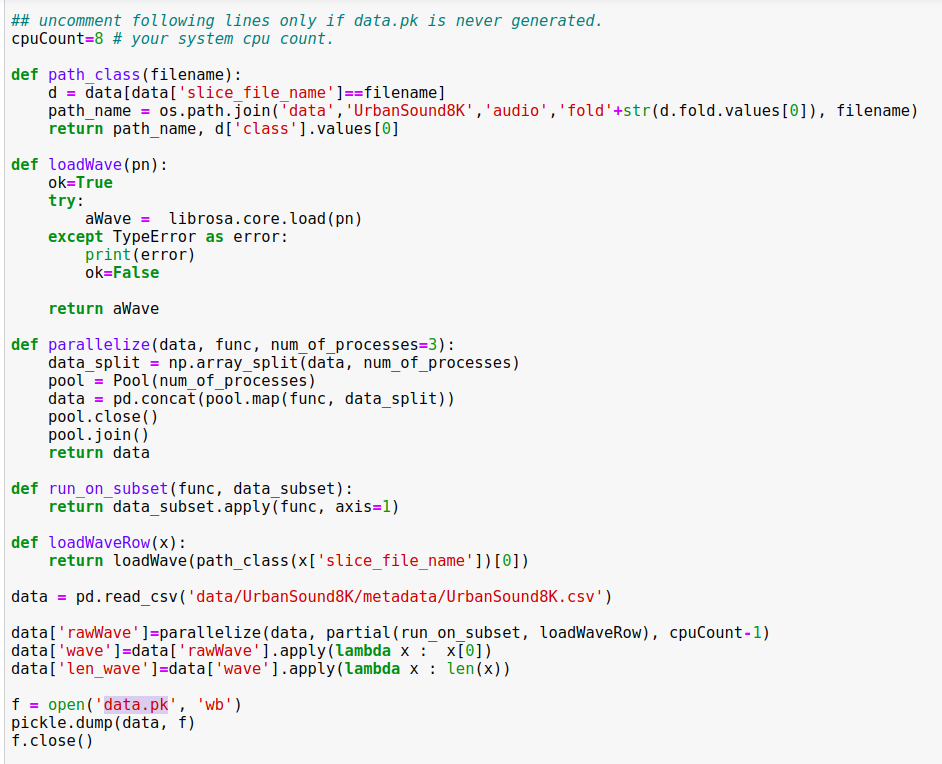
\includegraphics[width=7cm]{pic/data-loading.png}
	\end{tabular}}
	\caption{sound data loading, multiprocessing.\label{figure1}}
\end{figure}

As for sound duration that's less than 4 seconds, we concatenates the sound itself until it fills up the 4 seconds duration.

\begin{figure}[h]
	\centerline{\begin{tabular}{cc|c}
			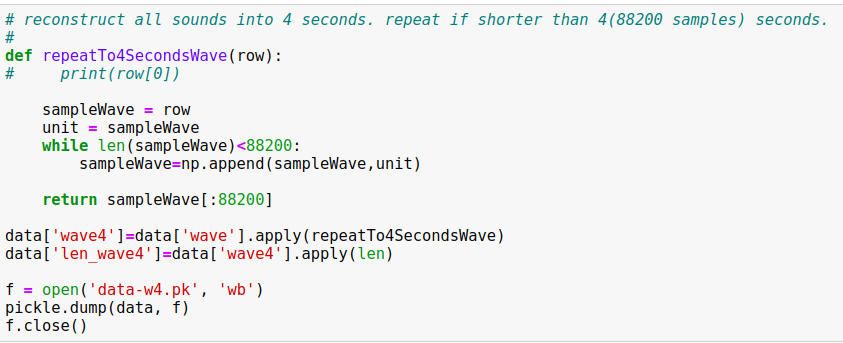
\includegraphics[width=7cm]{pic/self-repeatUntil4secs.png}
	\end{tabular}}
	\caption{self repeating to fill up to 4 seconds.\label{figure2}}
\end{figure}

We also plot and listen to a few gun shots and other sound files.
\begin{figure}[h]
	\centerline{\begin{tabular}{cc|c}
			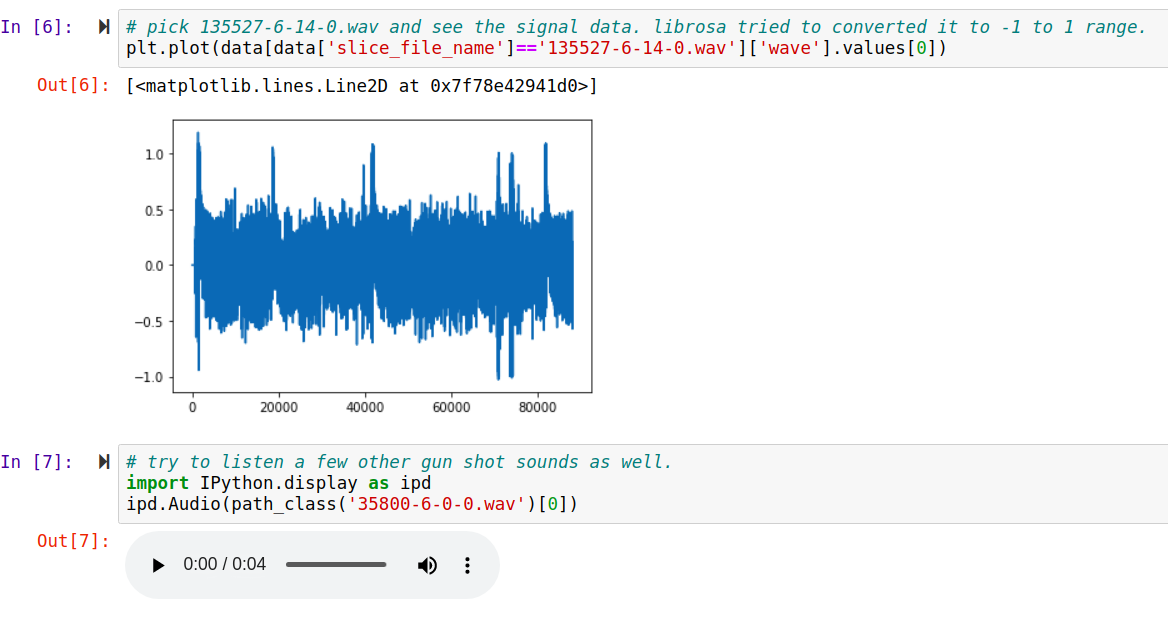
\includegraphics[width=7cm]{pic/plotAndPlaySounds.png}
	\end{tabular}}
	\caption{Plot and listen some sound files.\label{figure3}}
\end{figure}
There are ten classes in the data. They have different length of waves. After data extraction,need to ensure all the data has same size. We have use two methods to resize the waveform, one method is padding zero and another method is repeat the wave forms until the max. below figures show the plots before and after resizing use the two method.Blue color plots are the raw wave forms, green plots applied zero padding and yellow applied repeating.
\begin{figure}[!htb]
    \begin{tabular}{ccc}
        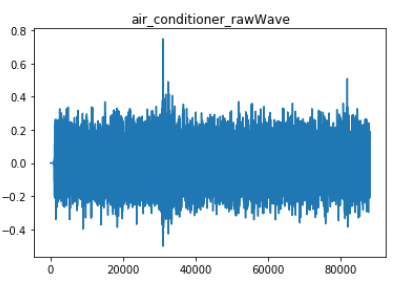
\includegraphics[width=2cm]{pic/AC_RW.png}
        &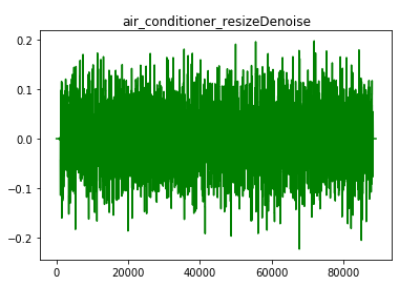
\includegraphics[width=2cm]{pic/AC_RSD.png}
        &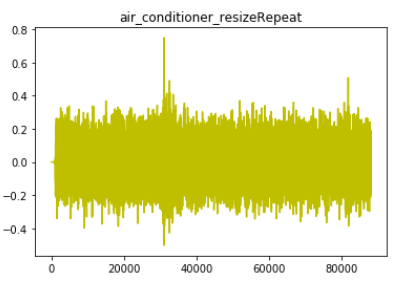
\includegraphics[width=2cm]{pic/AC_RSRP.png}\\
        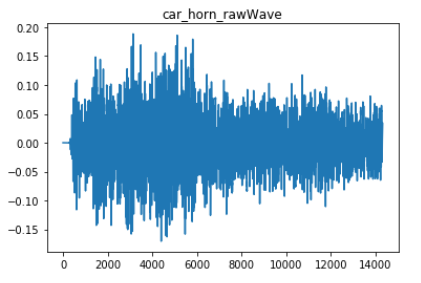
\includegraphics[width=2cm]{pic/CH_RW.png}
        &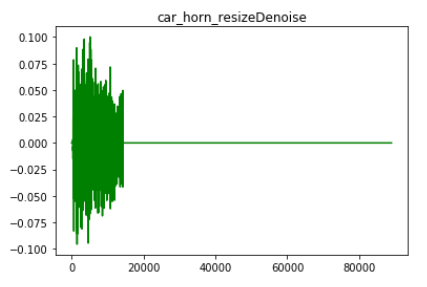
\includegraphics[width=2cm]{pic/CH_RSD.png}
        &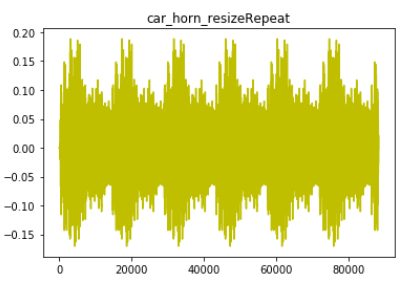
\includegraphics[width=2cm]{pic/CH_RSP.png}\\
        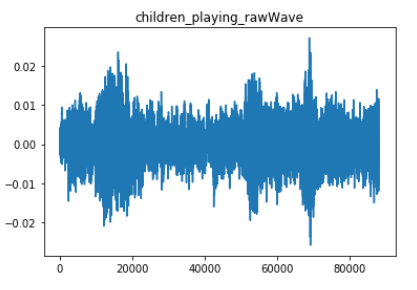
\includegraphics[width=2cm]{pic/CP_RW.png}
        &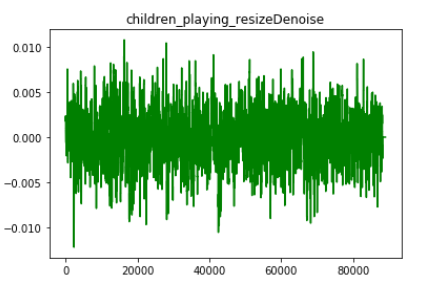
\includegraphics[width=2cm]{pic/CP_RSD.png}
        &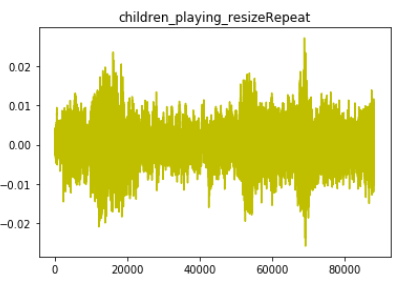
\includegraphics[width=2cm]{pic/CP_RSRP.png}\\
        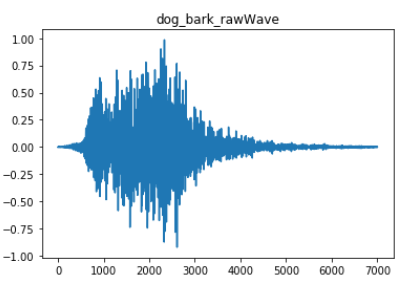
\includegraphics[width=2cm]{pic/DB_RW.png}
        &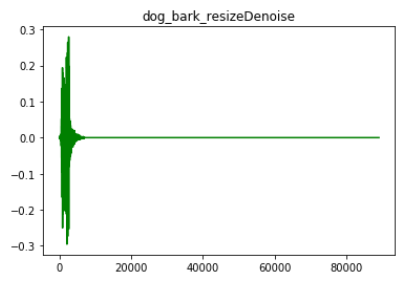
\includegraphics[width=2cm]{pic/DB_RSD.png}
        &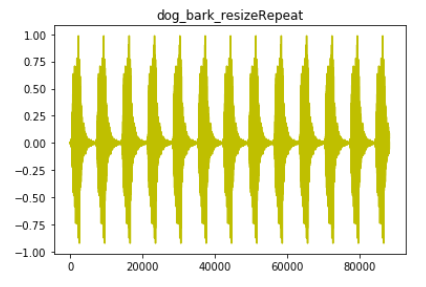
\includegraphics[width=2cm]{pic/DB_RSRP.png}\\
        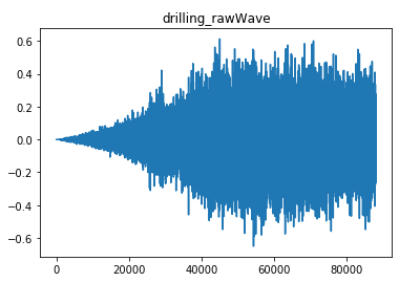
\includegraphics[width=2cm]{pic/DL_RW.png}
        &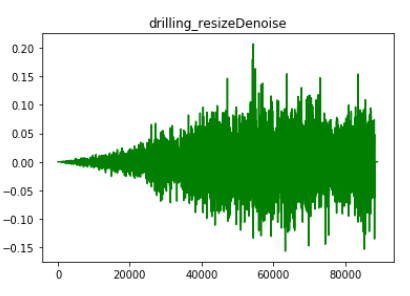
\includegraphics[width=2cm]{pic/DL_RSD.png}
        &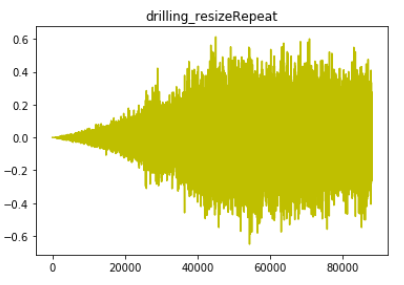
\includegraphics[width=2cm]{pic/DL_RSRP.png}\\
        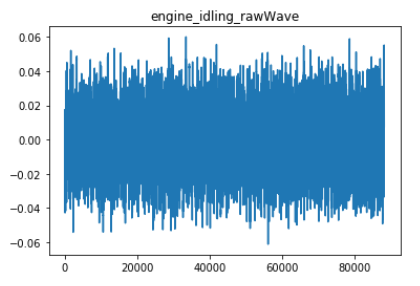
\includegraphics[width=2cm]{pic/EI_RW.png}
        &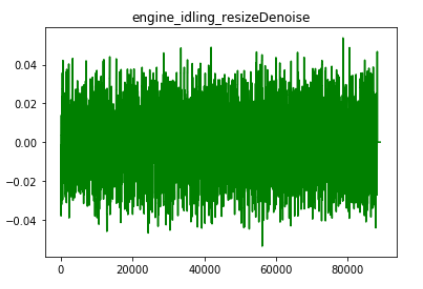
\includegraphics[width=2cm]{pic/EI_RSD.png}
        &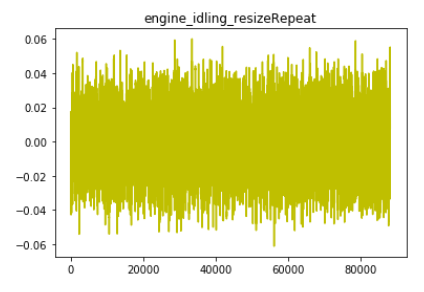
\includegraphics[width=2cm]{pic/EI_RSRP.png}\\
        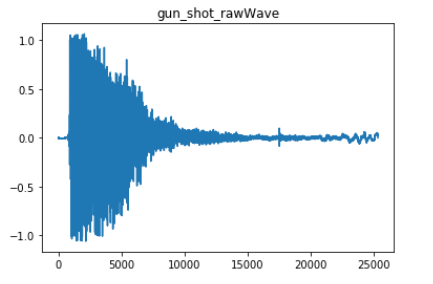
\includegraphics[width=2cm]{pic/GS_RW.png}
        &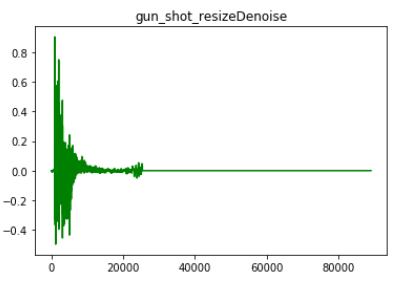
\includegraphics[width=2cm]{pic/GS_RSD.png}
        &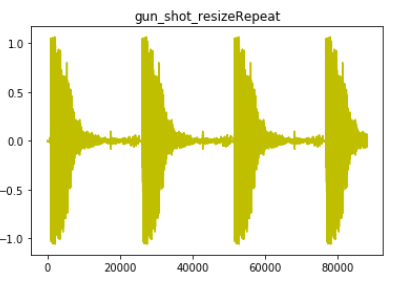
\includegraphics[width=2cm]{pic/GS_RSRP.png}\\
        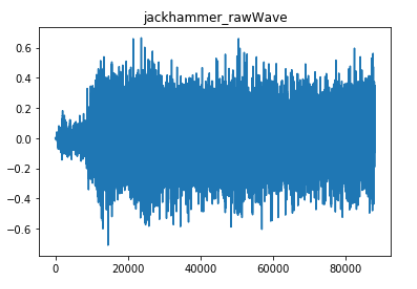
\includegraphics[width=2cm]{pic/JH_RW.png}
        &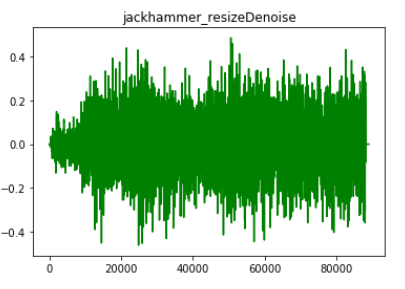
\includegraphics[width=2cm]{pic/JH_RSD.png}
        &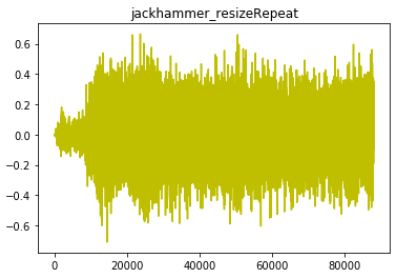
\includegraphics[width=2cm]{pic/JH_RSRP.png}\\
        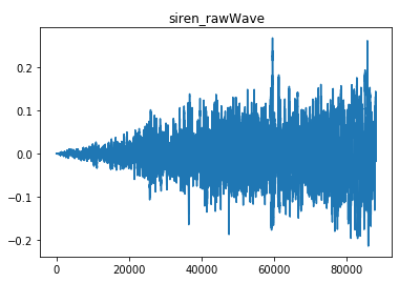
\includegraphics[width=2cm]{pic/SI_RW.png}
        &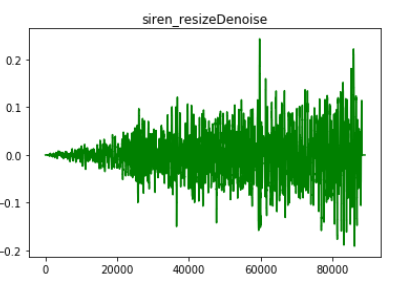
\includegraphics[width=2cm]{pic/SI_RSD.png}
        &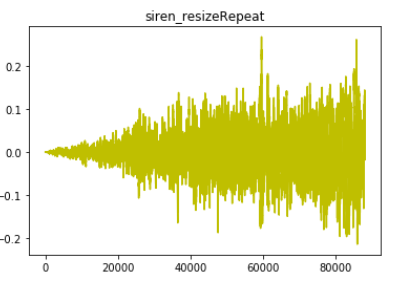
\includegraphics[width=2cm]{pic/SI_RSRP.png}\\
        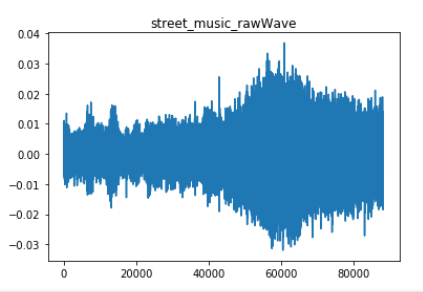
\includegraphics[width=2cm]{pic/SMC_RW.png}
        &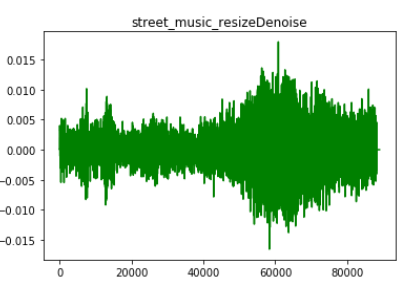
\includegraphics[width=2cm]{pic/SMC_RSD.png}
        &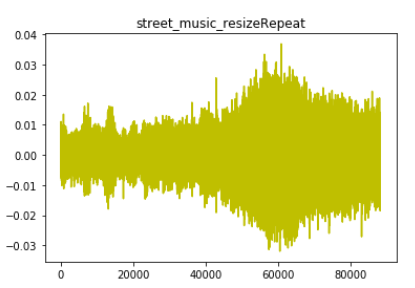
\includegraphics[width=2cm]{pic/SMC_RSRP.png}\\
    (raw wave) & (resize with zeros) &(resize with repeating)
    \end{tabular}
	\caption{sounds types, and 2 resizing schemes to 4 seconds.\label{figure4}}
\end{figure}

\newpage
\section{Experimental results}

\subsection{Conv1D deep neural network classification}
We constructed a four layers of Convolutional Neural Networks model for the wave data. the input data is 1D array which has 89007 features.
\begin{figure}[!htb]
    \begin{tabular}{c}
        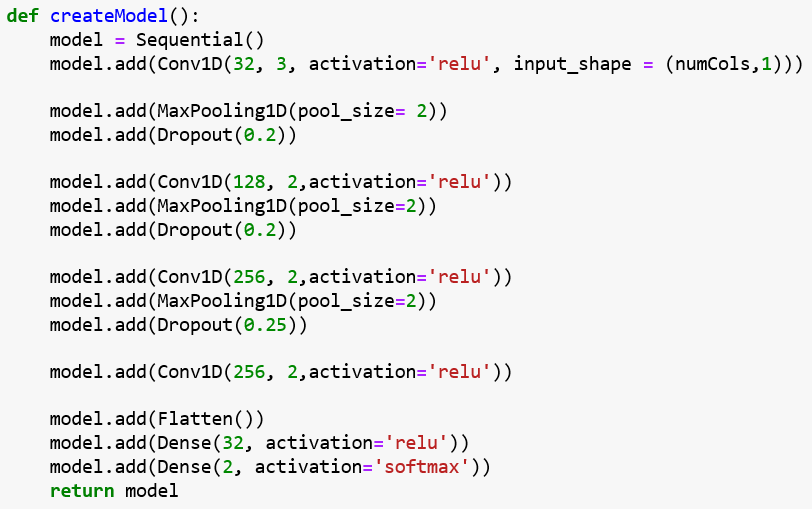
\includegraphics[width=8cm]{pic/CNN_Create.png}\\
    \end{tabular}
	\caption{model layers.\label{figure5}}
\end{figure}
\begin{figure}[!htb]
    \begin{tabular}{c}
        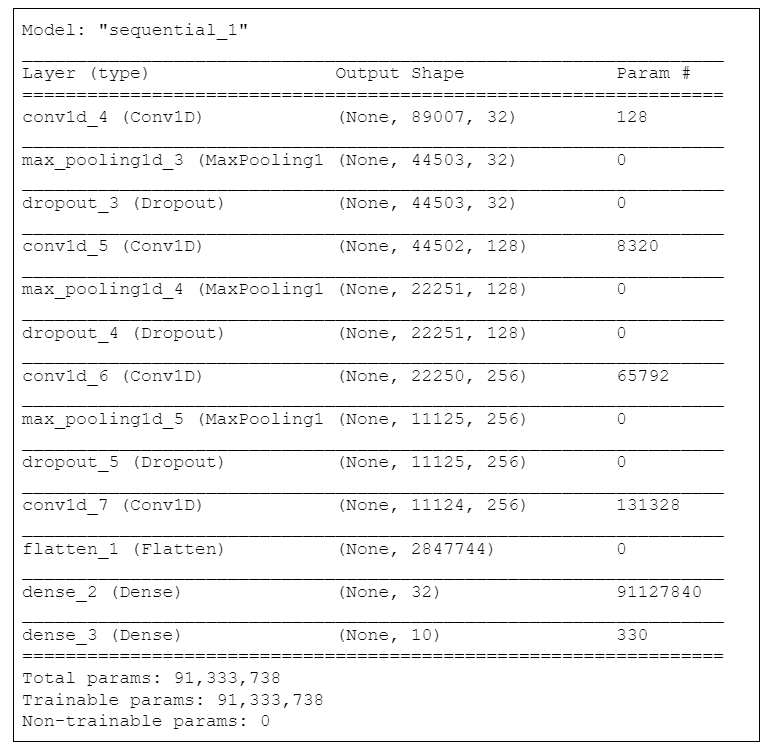
\includegraphics[width=8cm]{pic/CNN_Sum.png}\\
    \end{tabular}
	\caption{Model summary.\label{figure6}}
\end{figure}
\newpage
After data training and validation, the accuracy and the loss function showed training has good result but validation not.
\begin{figure}[!htb]
    \begin{tabular}{c}
        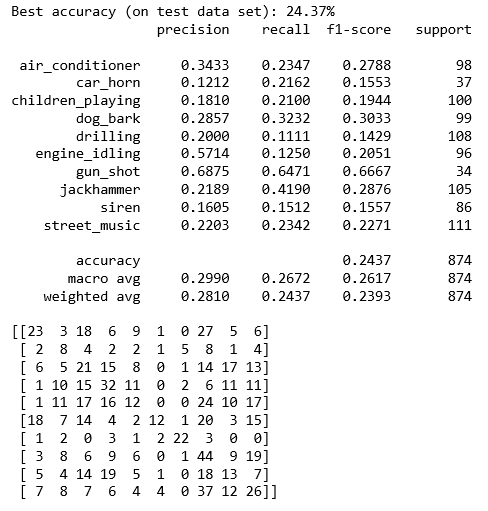
\includegraphics[width=7cm]{pic/CNN_Pm.png}\\
    \end{tabular}
	\caption{ CNN accuracy score and confusion matrix\label{figure7}}
\end{figure}
\newpage
We used a test data set did a prediction for the sounds classes, the result is 24.37\%. The gun shot prediction is 66.67\%.
\begin{figure}[!htb]
    \begin{tabular}{cc}
        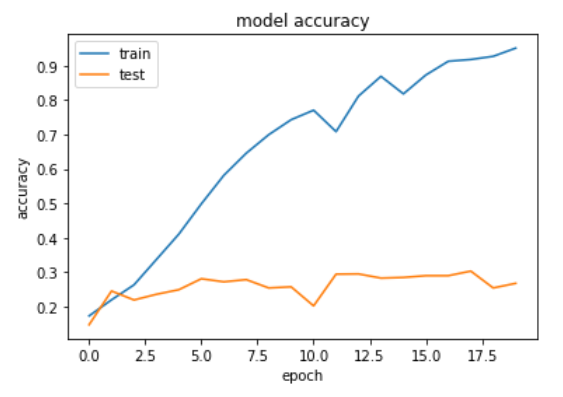
\includegraphics[width=4cm]{pic/CNN_ACC.png}
        &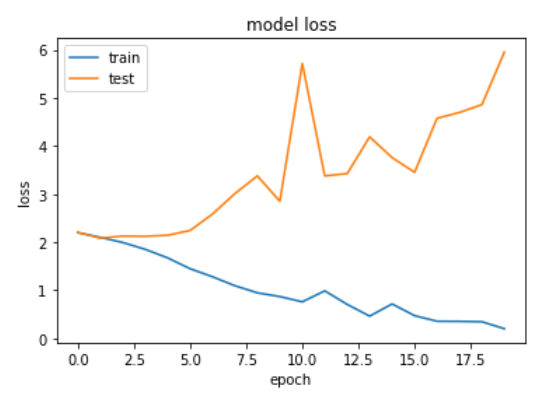
\includegraphics[width=4cm]{pic/CNN_LOSS.PNG}\\
    (model accuracy)&(model loss)
    \end{tabular}
	\caption{Model accuracy and model loss\label{figure8}}
\end{figure}
\newpage
Since our system is to check the dangerous sound (gun shot), we grouped non gun shot sounds as one class and gun shot as one class. Did another training for the data.

We used the test data set did a prediction for the sounds classes, the result is 97.14\%, but the gun shot prediction is 57.63\%.
\begin{figure}[!htb]
	\begin{tabular}{c}
		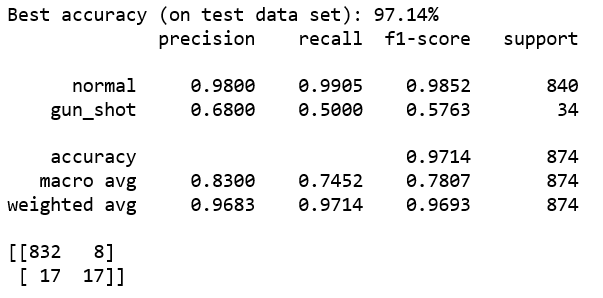
\includegraphics[width=7cm]{pic/CNN_Pm_V2.PNG}\\
	\end{tabular}
	\caption{CNN accuracy score and confusion matrix\label{figure9}}
\end{figure}

\begin{figure}[!htb]
	\begin{tabular}{cc}
		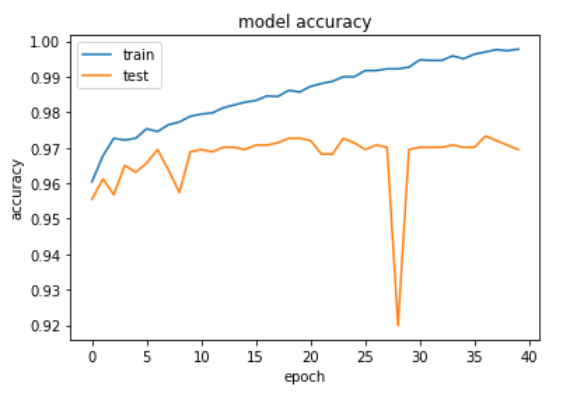
\includegraphics[width=4cm]{pic/CNN_ACC_V2.PNG}
		&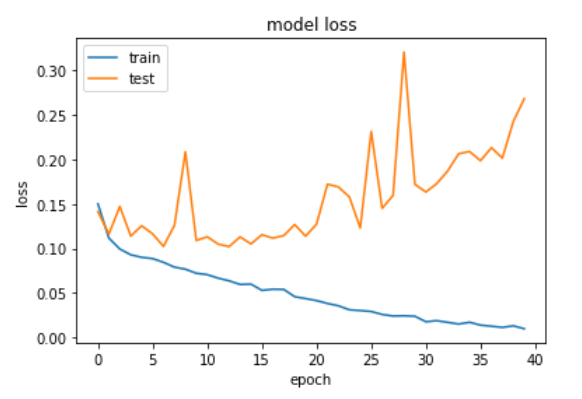
\includegraphics[width=4cm]{pic/CNN_Loss_V2.PNG}\\
		(model accuracy)&(model loss)
	\end{tabular}
	\caption{Model accuracy and model loss\label{figure10}}
\end{figure}
The accuracy of CNN is not good, we switch to other models.
Ref: https://github.com/XiaoyanYang2008/PRS-CA3-PoliceAlertSystem/blob/master/urbanSound\_CNN.ipynb

\newpage
\subsection{Autoencoder anomaly detection}
Based on 4 seconds self-repeat sound, we construct autoencoder and train with sounds sample without gun shots. Below is the code snipet for the autoencoder network.

\begin{figure}[ht]
	\centerline{\begin{tabular}{c}
			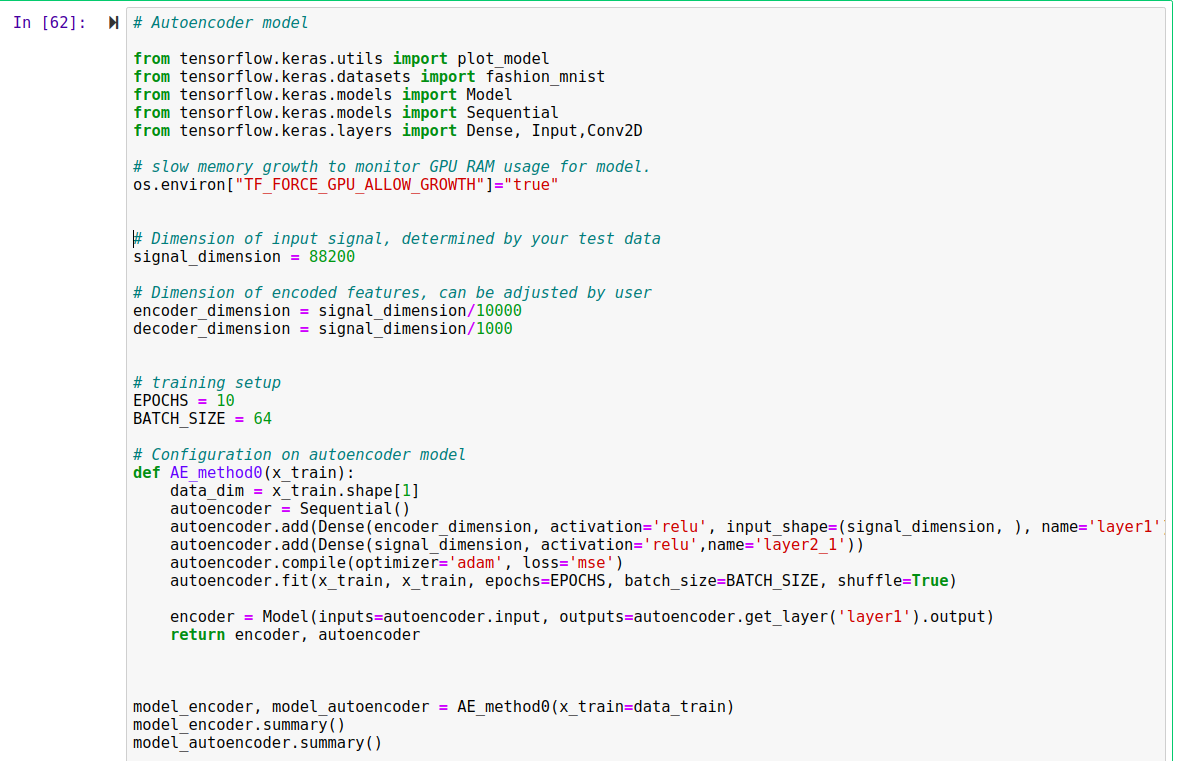
\includegraphics[width=7cm]{pic/auto-encoder-network.png}
	\end{tabular}}
	\caption{Autoencoder network.\label{figure11}}
\end{figure}
\begin{figure}[ht]
	\centerline{\begin{tabular}{c}
			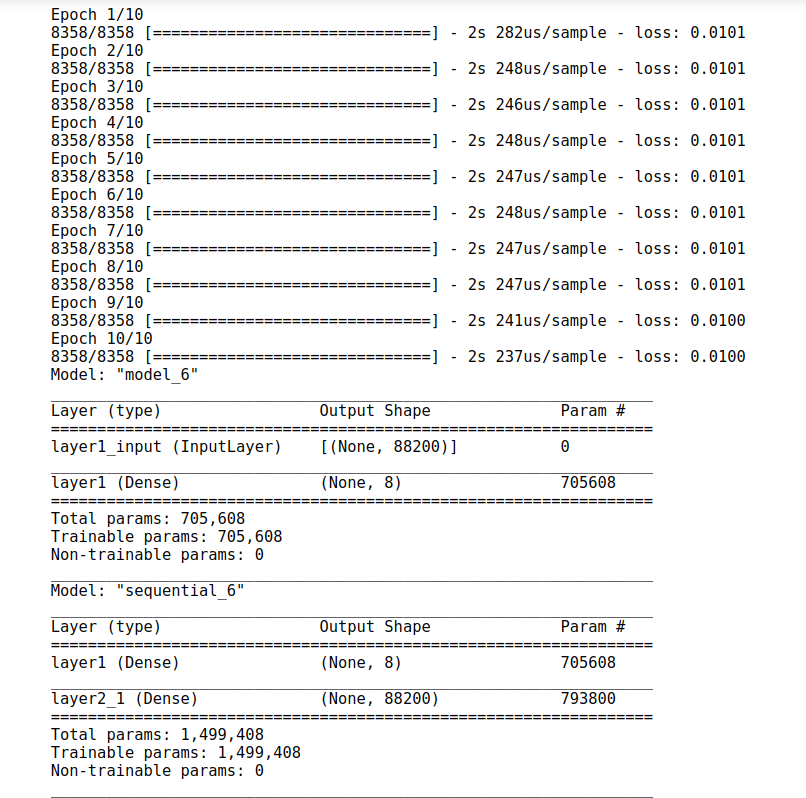
\includegraphics[width=7cm]{pic/autoencoder-training-summary.png}
	\end{tabular}}
	\caption{Autoencoder network training and its structure\label{figure12}}
\end{figure}

By training autoencoder network with non gun shots sound data, we hope that gun shots sound will be recognized as anomaly to the network. Due to 4 seconds and sampling rate of 22kHz, our data will be 1D arrary of 88.200k samples. From Fig. \ref{figure12}, layer1, which is the innermost layer of undercomplete autoencoder neural network, it has only 8 neurons.

The code to analyse performance of training data and gun shot(noise, test) anomaly detection is as below. 

\begin{figure}[ht]
	\centerline{\begin{tabular}{c}
			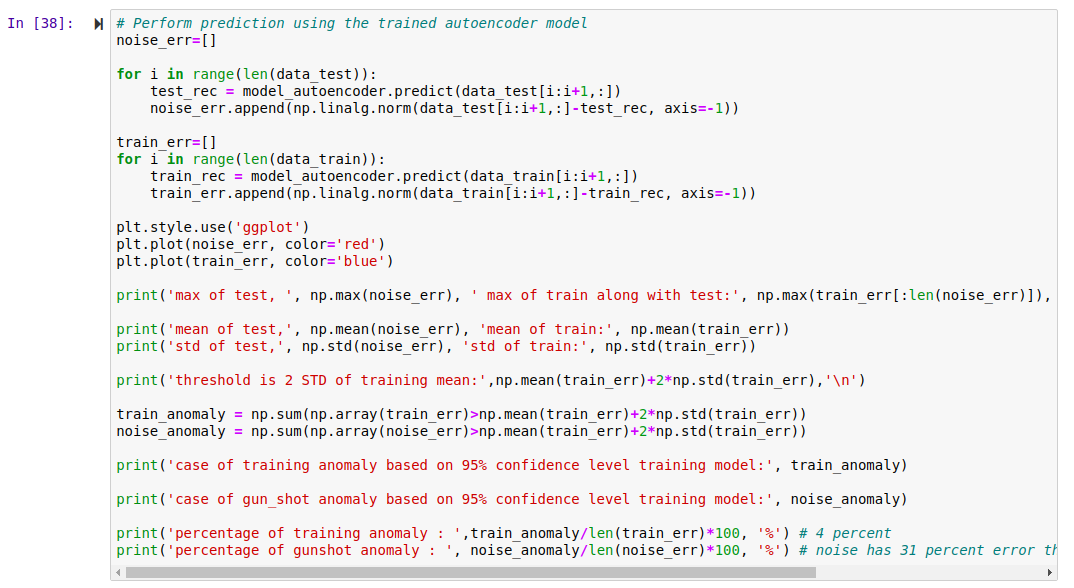
\includegraphics[width=7cm]{pic/autoencoded-8-31.png}
	\end{tabular}}
	\caption{Auto encoder performance analysis code snipet\label{figure13}}
\end{figure}
Based on the errors collected from network prediction on training data and gun shot data, we calculate mean and standard deviation, std. With 95\% confidence level as guideline, we set the threshold to mean+2*std, which is 62.17.

\newpage

\begin{figure}[ht]
	\centerline{\begin{tabular}{c}
			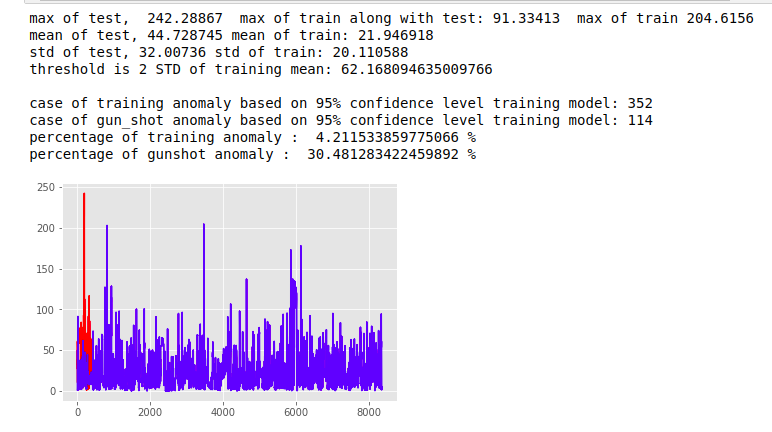
\includegraphics[width=7cm]{pic/autoencoder-8-31-result.png}
	\end{tabular}}
	\caption{Autoencoder performance analysis\label{figure14}}
\end{figure}

With threshold of 62.17 in Fig. \ref{figure14}, we found out that only 4.2\% of training data is anomaly, whereas gun shot data anomaly rate is about 30.48\% at 95\% confidence level. 

Though the performance is not amazing compared to other methods in later parts of experiements. It is interesting that autoencoder can detect anomaly even within its own training data. It is useful that when we don't have much labelled data but unsupervised learning like this, helps to point out anomaly.


We also notice another counter intuitive perspective about autoencoder. For neural network, more neurons tends to performance better.
\begin{figure}[ht]
	\centerline{\begin{tabular}{c}
			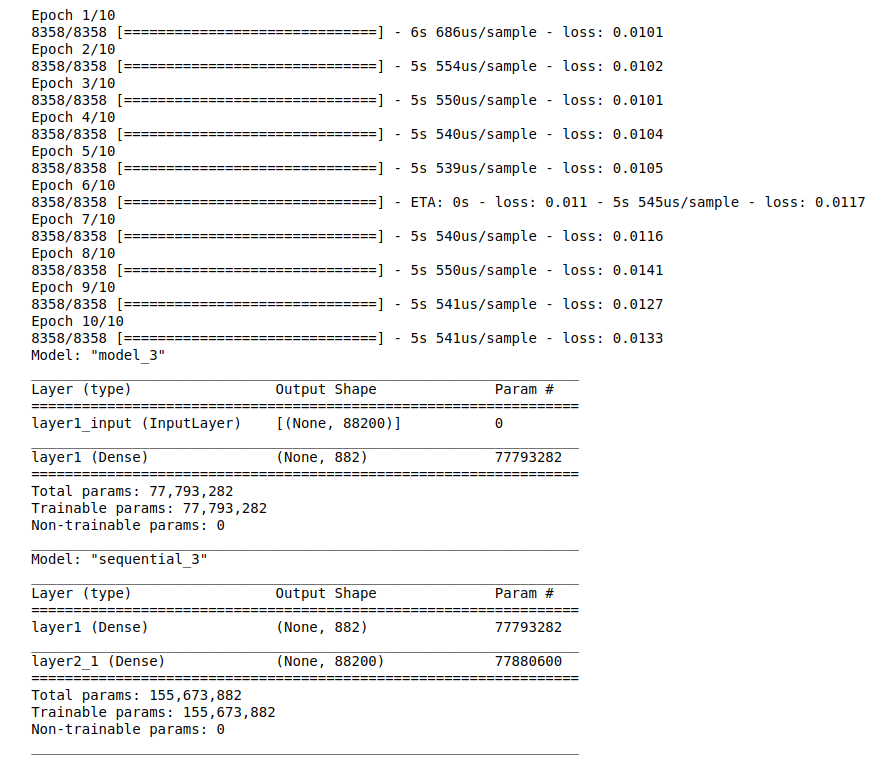
\includegraphics[width=7cm]{pic/autoencoder-800.png}
	\end{tabular}}
	\caption{Autoencoder with 800 innermost layer \label{figure15}}
\end{figure}
However, this is not the case for autoencoder. We configure 100x more neurons for innermost layer, and spend more times on compute. And here is the performance of the network,
\begin{figure}[ht]
	\centerline{\begin{tabular}{c}
			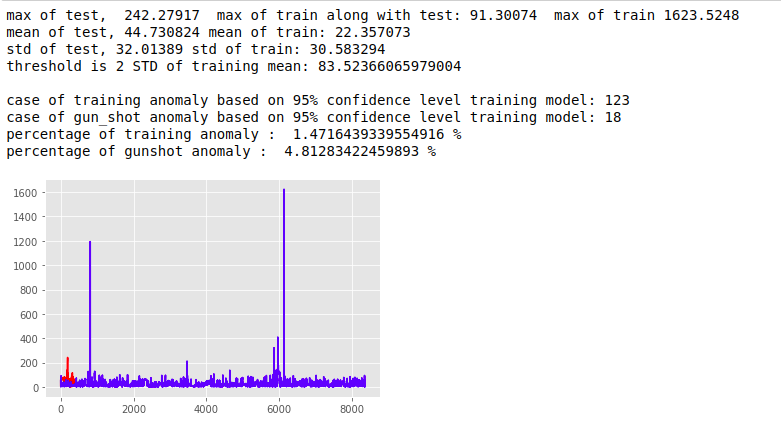
\includegraphics[width=7cm]{pic/autoencoder-800-performance.png}
	\end{tabular}}
	\caption{Performance of Autoencoder with 800 innermost layer \label{figure16}}
\end{figure}

The performance on gunshot anomaly detection is only 4.8\%, which is only 16\% of 8 neurons network. Therefore, more under-complete autoencoder network likely pressing the neural network to perform better.
ref: https://github.com/XiaoyanYang2008/PRS-CA3-PoliceAlertSystem/blob/master/urbanSound-autoencoder-normal.ipynb

\newpage
\subsection{LSTM neural network classifcation}
Long short-term memory(LSTM) neural network is another typical tool to handle 1D time series data. Below is the network structure we deployed for classification model training. Due to slow training performance in LSTM, we deployed conv1D layers and multiple MaxPooling1D(16) to reduce data while keeping peak values to LSTM layer.
\begin{figure}[ht]
	\centerline{\begin{tabular}{c}
			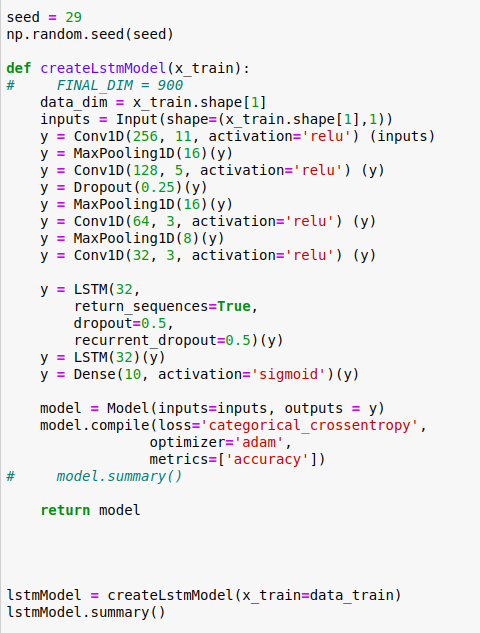
\includegraphics[width=7cm]{pic/lstm-code.png}
	\end{tabular}}
	\caption{LSTM network structures \label{figure17}}
\end{figure}

\begin{figure}[ht]
	\centerline{\begin{tabular}{c}
			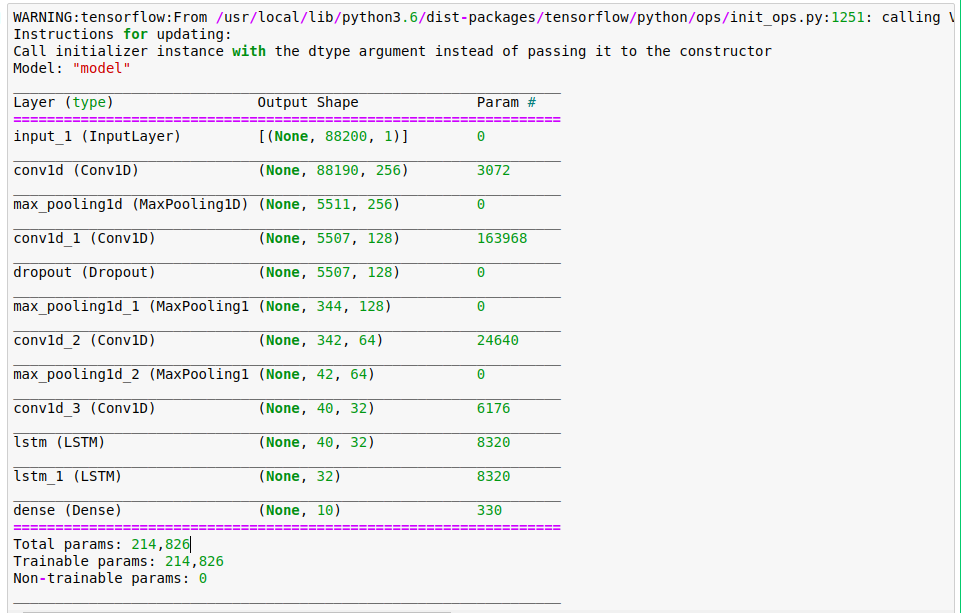
\includegraphics[width=7cm]{pic/lstm-layers.png}			
	\end{tabular}}
	\caption{LSTM network layers \label{figure18}}
\end{figure}
\newpage
From the initial training, even with maxPooling1D(16), we roughly estimated that LSTM training takes more epochs to improve.
\begin{figure}[ht]
	\centerline{\begin{tabular}{c}
			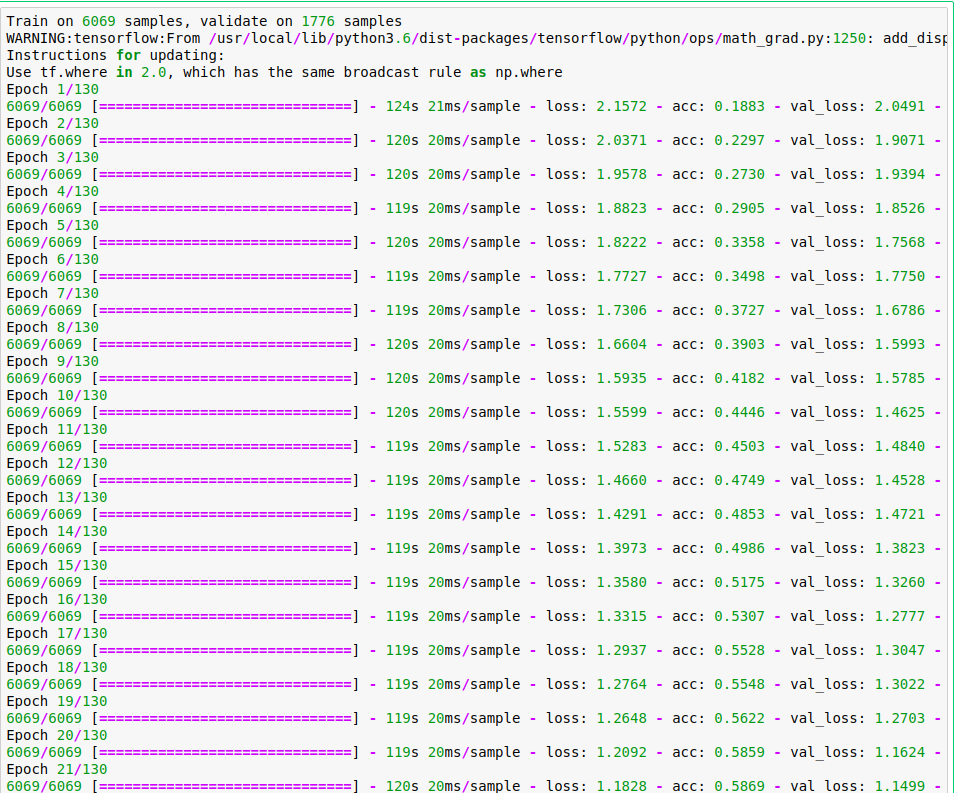
\includegraphics[width=7cm]{pic/lstm-training-start.png}			
	\end{tabular}}
	\caption{LSTM training, beginging phase \label{figure19}}
\end{figure}

\begin{figure}[ht]
	\centerline{\begin{tabular}{c}
			\includegraphics[width=7cm]{pic/lstm-training-end.png}			
	\end{tabular}}
	\caption{LSTM training, ending phase \label{figure19}}
\end{figure}
\newpage

And based on following chart, LSTM training indeed taking more time to reach plateu by around 100 epochs, which is way more epochs than autoencoder as well as Conv1D network. This is likely due to slow propagation of feedback via memory unit cell in LSTM.
\begin{figure}[ht]
	\centerline{\begin{tabular}{c}
			\includegraphics[width=7cm]{pic/lstm-training-graph.png}\\
			(green color is validation)		
	\end{tabular}}
	\caption{LSTM training accuracy and loss \label{figure19}}
\end{figure}

From figure below, we observe that our LSTM model achieve 78.69\% accuracy on various sound classification. For gun shot sound, the F1 score is 0.8732, which is 2nd best classifiable sounds. Car\_horn and drilling sound classification tasks dragged down the overall model performance.

\begin{figure}[ht]
	\centerline{\begin{tabular}{c}
			\includegraphics[width=7cm]{pic/lstm-accuracy.png}\\
	\end{tabular}}
	\caption{LSTM classification performance \label{figure20}}
\end{figure}

Ref: https://github.com/XiaoyanYang2008/PRS-CA3-PoliceAlertSystem/blob/master/urbanSound-LSTM.ipynb


\newpage
\subsection{MFCC representation and neural network classification}

In the earlier model using CNN, we were extracting each audio file as a floating point time series to train our model. However, this method does not capture envelope of the short time power spectrum characteristics of the audio. As such, we decided to use MFCC feature extraction function in librosa as per \cite{MikeSmalesSoundClassificationusingDeepLearning}. However, we are different in that we MFCC our audio file and load the mean of each MFCC bin, into our Neural network (NN) model to see if model accuracy improved.


\begin{center}
\begin{tabular}{ |l| }
 \hline
 num\_epochs = 100 \\
 num\_batch\_size = 32 \\
 seed = 29 \\
 np.random.seed(seed) \\
 \hline
\end{tabular}
\end{center}

Based on the code that we referenced from , we started our training by extracting MFCC feature of our audio file into 40 "bins".

\begin{figure}[ht]
	\centerline{\begin{tabular}{c}
			\includegraphics[width=7cm]{pic/MFCC_extract_audio_features_from.png}
	\end{tabular}}
\end{figure}

Let's take a look at MFCC spectrogram of 2 audio files, namely Children Playing and Gun Shot.
\newpage
\begin{figure}[ht]
	\centerline{\begin{tabular}{c}
			\includegraphics[width=7cm]{pic/MFCC_children_play_spectrogram.png}
	\end{tabular}}
	\caption{Spectrogram of Children Playing audio \label{figure18}}
\end{figure}

\begin{figure}[ht]
	\centerline{\begin{tabular}{c}
			\includegraphics[width=7cm]{pic/MFCC_gunshot_spectrogram.png}
	\end{tabular}}
	\caption{Spectrogram of Gun Shot audio \label{figure19}}
\end{figure}


You can see these 2 audio files have very different spectrogram where
gunshot has a high pitch at the beginning of the audio file. With that,
we will start training our model.


As our class label is categorical value, we need to do a one time label encoding to cover them to numeric for our model to work.

\begin{center}
\begin{tabular}{ |l| }
 \hline
 le = LabelEncoder() \\
 yy = to\_categorical(le.fit\_transform(y)) \\
 \hline
\end{tabular}
\end{center}


We split the dataset to 70\%, 20\% and 10\% for training, validation and testing purpose respectively.

\begin{center}
\begin{tabular}{ |l| }
 \hline
    mask = np.random.rand(len(data)) \\
    train\_mask = mask < 0.7 \\
    validation\_mask = np.logical\_and(mask > 0.7, mask < 0.9) \\
    test\_mask = mask > 0.9 \\
 \hline
\end{tabular}
\end{center}


For the training, we are using a CNN model. As the model is to predict
and classify to 10 audio classes, our model final output layer will be
10.

\begin{center}
\begin{tabular}{ |l| }
 \hline
model =  Sequential() \\
model.add(Dense(256, input\_shape=(n\_mfcc,))) \\
model.add(Activation("relu")) \\
model.add(Dropout(0.25)) \\
model.add(Dense(64)) \\
model.add(Activation("relu")) \\
model.add(Dropout(0.25)) \\
model.add(Dense(128)) \\
model.add(Activation("relu")) \\
model.add(Dropout(0.25)) \\
model.add(Dense(256)) \\
model.add(Activation("relu")) \\
model.add(Dropout(0.25)) \\
model.add(Dense(512)) \\
model.add(Activation(\"relu")) \\
model.add(Dropout(0.5)) \\
model.add(Dense(yy.shape[1])) \\
model.add(Activation("softmax")) \\
model.compile(loss="categorical\_crossentropy", \\
            metrics=["accuracy"], optimizer="adam") \\
model.summary() \\
\\
history=  model.fit(x\_train, y\_train, \\
            batch\_size=num\_batch\_size, \\
            epochs=num\_epochs, \\
            validation\_data=(x\_valid, y\_valid), \\
            callbacks=[checkpointer], \\
            verbose=1)\\
 \hline
\end{tabular}
\end{center}


\begin{figure}[ht]
	\centerline{\begin{tabular}{c}
			\includegraphics[width=7cm]{pic/MFCC40_CNN_Model.png}
	\end{tabular}}
	\caption{NN Model for n\_mfcc=40 \label{figure20}}
\end{figure}

\begin{center}
\begin{tabular}{ |l| }
 \hline
score=model.evaluate(x\_train,y\_train,verbose=0) \\
score=model.evaluate(x\_test,y\_test,verbose=0) \\
\\
Training Accuracy:  0.92509854\\
Testing Accuracy:  0.8630435\\
 \hline
\end{tabular}
\end{center}

\begin{figure}[ht]
	\centerline{\begin{tabular}{c}
			\includegraphics[width=7cm]{pic/MFCC40_Epoch_Accuracy.png}
	\end{tabular}}
	\caption{Accuracy for NN Model with n\_mfcc=40 \label{figure21}}
\end{figure}

\begin{figure}[ht]
	\centerline{\begin{tabular}{c}
			\includegraphics[width=7cm]{pic/MFCC40_Epoch_Loss.png}
	\end{tabular}}
	\caption{Loss for NN Model with n\_mfcc=40 \label{figure22}}
\end{figure}

\begin{figure}[ht]
	\centerline{\begin{tabular}{c}
			\includegraphics[width=7cm]{pic/MFCC40_CNN_Model_Test_Accuracy_Grid.png}
	\end{tabular}}
\end{figure}

\newpage
\begin{figure}[ht]
	\centerline{\begin{tabular}{c}
			\includegraphics[width=7cm]{pic/MFCC40_confusion_matrix.png}
	\end{tabular}}
	\caption{Confusion Matrix for NN Model with n\_mfcc=40 \label{figure23}}
\end{figure}



Using MFCC features of the audio files for training, has improved the model overall accuracy, from 24.26\% to 86.30\%. And looking at the confusion matrix, we can see a small number of audio files were missed classified. Let's take a quick look some of them.

\begin{figure}[ht]
	\centerline{\begin{tabular}{c}
			\includegraphics[width=7cm]{pic/MFCC_Drilling_spectogram.png}
	\end{tabular}}
	\caption{Spectrogram for a Drilling audio \label{figure24}}
\end{figure}

\begin{figure}[ht]
	\centerline{\begin{tabular}{c}
			\includegraphics[width=7cm]{pic/MFCC_Car_Horn_spectogram.png}
	\end{tabular}}
	\caption{Spectrogram for a Drilling audio \label{figure25}}
\end{figure}

\newpage
With the classifier model, we are going to test it using a audio file where we created by overlaying a gunshot audio on top of a children playing audio at 6.5 seconds. Here is what the MFCC spectrogram looks like:


\begin{figure}[ht]
	\centerline{\begin{tabular}{c}
			\includegraphics[width=7cm]{pic/MFCC_MixedAudio_spectrogram.png}
	\end{tabular}}
	\caption{Spectrogram for a mixed audio \label{figure26}}
\end{figure}


The predicted class is: children\_playing

\begin{center}
\begin{tabular}{ |l|r| }
 \hline
air\_conditioner &  0.03\% \\
car\_horn            &  0.02\% \\
children\_playing    & 69.43\% \\
dog\_bark            & 15.47\% \\
drilling            &  0.48\% \\
engine\_idling       &  0.45\% \\
gun\_shot            & 11.01\% \\
jackhammer          &  0.00\% \\
siren               &  2.32\% \\
street\_music        &  0.80\% \\
 \hline
\end{tabular}
\end{center}


Using this current model (with overall accuracy of 86.30\%), we were about to identify the presence of gunshot sound within the children playing. But we wonder if we can improve the model accuracy further by increasing the number of MFCC bins. Thus next, we will explore this parameter.


Our approach is to increase the MFCC bin size from 40 to 60 to extract more features from the audio file. And due to the increase in features, we needed more epochs to train the model.


\begin{center}
\begin{tabular}{ |l| }
 \hline
    n\_mfcc = 60 \\
    num\_epochs = 200 \\
    num\_batch\_size = 64 \\
 \hline
\end{tabular}
\end{center}


\begin{figure}[ht]
	\centerline{\begin{tabular}{c}
			\includegraphics[width=7cm]{pic/MFCC60_CNN_Model.png}
	\end{tabular}}
	\caption{NN Model for n\_mfcc=60 \label{figure27}}
\end{figure}

\begin{center}
\begin{tabular}{ |l| }
 \hline
Training Accuracy:  0.97848225 \\
Testing Accuracy:  0.90434784 \\
 \hline
\end{tabular}
\end{center}


\begin{figure}[ht]
	\centerline{\begin{tabular}{c}
			\includegraphics[width=7cm]{pic/MFCC60_Epoch_Accuracy.png}
	\end{tabular}}
	\caption{Accuracy for NN Model with n\_mfcc=60 \label{figure28}}
\end{figure}


\begin{figure}[ht]
	\centerline{\begin{tabular}{c}
			\includegraphics[width=7cm]{pic/MFCC60_Epoch_Loss.png}
	\end{tabular}}
	\caption{Loss for NN Model for n\_mfcc=60 \label{figure29}}
\end{figure}

\newpage
\begin{figure}[ht]
	\centerline{\begin{tabular}{c}
			\includegraphics[width=7cm]{pic/MFCC60_CNN_Model_Test_Accuracy_Grid.png}
	\end{tabular}}
\end{figure}


\begin{figure}[ht]
	\centerline{\begin{tabular}{c}
			\includegraphics[width=7cm]{pic/MFCC60_Confusion_Matrix.png}
	\end{tabular}}
	\caption{Confusion Matrix for model using n\_mfcc=60 \label{figure30}}
\end{figure}

\newpage
With the increase in the number of MFCC bins, we were able to improve the overall model accuracy from 86.30\% to 90.40\%. An improvement in accuracy by 7.23\% with 2.50\% increase in total params in the model.



The predicted class is: children\_playing

\begin{center}
\begin{tabular}{ |l|r| }
 \hline
air\_conditioner &  0.08\% \\
car\_horn            &  0.00\% \\
children\_playing    & 98.15\% \\
dog\_bark            & 0.52\% \\
drilling            &  0.11\% \\
engine\_idling       &  0.14\% \\
gun\_shot            & 0.85\% \\
jackhammer          &  0.01\% \\
siren               &  0.06\% \\
street\_music        &  0.07\% \\
 \hline
\end{tabular}
\end{center}


We observed that the improvement in model accuracy has increase the prediction probability for the children playing class. And the second highest probability is the gun shot sound that we have overlay-ed on top of children playing.


Ref: https://github.com/XiaoyanYang2008/PRS-CA3-PoliceAlertSystem/blob/master/BEST\_urbanSound\_CNN\_MFCC60.ipynb






%\begin{equation}\label{equation block model}
%B_{r,c}=\sum\{f(i,j)|(i,j)\in \Omega_{r,c}\}.
%\end{equation}
%\begin{equation}\label{equation 1}
%\sum_{x}=a+b+\hat{c},
%\end{equation}

%An inline equation is $a+b=c$. An example of two-column figure is provided in Figure \ref{figure1}, and the single-column figures is provided in Figure \ref{figure2}.

%\begin{figure*}[tbh]\includegraphics[width=15cm]{iss.png}
%    \caption{Test figure (two-column).\label{figure1}}
%\end{figure*}


\newpage
\section{Conclusions}
\label{sec:conclusions}

% Summarize your key results. What are limitations of your approach? Suggest ideas for future extensions of your ideas.
With findings above, we summarize our classification performance as following table:

\begin{table}[tbh]
	\caption{The performance comparison.}\label{table1} \centerline{
		\begin{tabular}{clc|r}
			\hline\hline
			Approaches & Classification Accuracy\\
			Conv1D & $0.2437$\\\hline
			Autoencoder & $0.3048$ \\\hline
			LSTM & $0.7869$ \\\hline
			MFCC NN & $0.9043$ \\\hline
		\end{tabular}
	}
\end{table}

From experiments, we can conclude following ideas:
1. MFCC converts time series signal to frequency domain, which in this case, well suit for classification.
2. But if time series signal isn't well suit, as maybe it doesn't have clear frequency bands within the signal, then LSTM probably can handle those time series signals well enough. At least, it is able to handle time series signal without special handling in this case.
3. autoencoder is interesting to use especially when no clear data labelling.
4. conv1d isn't performed well, if compared to LSTM, which means that memory unit designed in LSTM does have advantage over normal convolution network.




\bibliographystyle{IEEEbib}
\bibliography{references}

\end{document}
